\documentclass[tikz,border=2mm]{standalone}
\usepackage{tikz}
\usetikzlibrary{arrows,positioning}
\usepackage{pgfplots}
\usepackage{amsmath,mathtools}
\usepgfplotslibrary{fillbetween}
\pgfplotsset{compat=1.17}
\begin{document}
% Picture 1: simulated data ZOOMED IN 
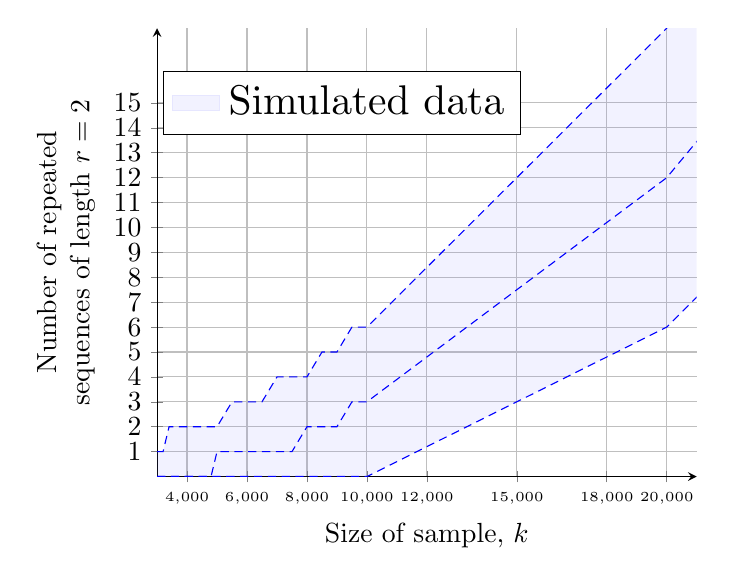
\begin{tikzpicture}
\begin{axis}[
    axis lines=left, %xtick=\empty, ytick=\empty.
    grid=both,
    xmin = 3000,
    xmax = 21000,
    scaled x ticks = false,
    xticklabel style = {font=\tiny},
    xtick = {2000,4000,6000,8000,10000,12000,15000,18000,20000},
    ytick = {1,...,15},
    %xticklabels = {$2000$,$5000$,$10,000$,$20,000$,$30,000$,$40,000$},
    ylabel style = {align=center},
	xlabel = {Size of sample, $k$},
        ylabel = {Number of repeated\\ sequences of length $r=2$},
    legend style={at={(axis cs:3200,15)},anchor=west,cells={align=center},nodes={scale=1.5}},
]
% Include the simulated data
\addplot[forget plot,densely dashed,color=blue,name path=down]coordinates {
	(3000.0000	,	0.0000)
	(3200.0000	,	0.0000)
	(3400.0000	,	0.0000)
	(3600.0000	,	0.0000)
	(3800.0000	,	0.0000)
	(4000.0000	,	0.0000)
	(4200.0000	,	0.0000)
	(4400.0000	,	0.0000)
	(4600.0000	,	0.0000)
	(4800.0000	,	0.0000)
	(5000.0000	,	0.0000)
	(5500.0000	,	0.0000)
	(6000.0000	,	0.0000)
	(6500.0000	,	0.0000)
	(7000.0000	,	0.0000)
	(7500.0000	,	0.0000)
	(8000.0000	,	0.0000)
	(8500.0000	,	0.0000)
	(9000.0000	,	0.0000)
	(9500.0000	,	0.0000)
	(10000.0000	,	0.0000)
	(20000.0000	,	6.0000)
	(30000.0000	,	18.0000)
	(40000.0000	,	36.0000)
	(50000.0000	,	61.0000)
};
\addplot[forget plot,densely dashed,color=blue]coordinates {
	(3000.0000	,	0.0000)
	(3200.0000	,	0.0000)
	(3400.0000	,	0.0000)
	(3600.0000	,	0.0000)
	(3800.0000	,	0.0000)
	(4000.0000	,	0.0000)
	(4200.0000	,	0.0000)
	(4400.0000	,	0.0000)
	(4600.0000	,	0.0000)
	(4800.0000	,	0.0000)
	(5000.0000	,	1.0000)
	(5500.0000	,	1.0000)
	(6000.0000	,	1.0000)
	(6500.0000	,	1.0000)
	(7000.0000	,	1.0000)
	(7500.0000	,	1.0000)
	(8000.0000	,	2.0000)
	(8500.0000	,	2.0000)
	(9000.0000	,	2.0000)
	(9500.0000	,	3.0000)
	(10000.0000	,	3.0000)
	(20000.0000	,	12.0000)
	(30000.0000	,	26.5000)
	(40000.0000	,	47.0000)
	(50000.0000	,	74.0000)
};
\addplot[forget plot,densely dashed,color=blue,name path=up]coordinates {
	(3000.0000	,	1.0000)
	(3200.0000	,	1.0000)
	(3400.0000	,	2.0000)
	(3600.0000	,	2.0000)
	(3800.0000	,	2.0000)
	(4000.0000	,	2.0000)
	(4200.0000	,	2.0000)
	(4400.0000	,	2.0000)
	(4600.0000	,	2.0000)
	(4800.0000	,	2.0000)
	(5000.0000	,	2.0000)
	(5500.0000	,	3.0000)
	(6000.0000	,	3.0000)
	(6500.0000	,	3.0000)
	(7000.0000	,	4.0000)
	(7500.0000	,	4.0000)
	(8000.0000	,	4.0000)
	(8500.0000	,	5.0000)
	(9000.0000	,	5.0000)
	(9500.0000	,	6.0000)
	(10000.0000	,	6.0000)
	(20000.0000	,	18.0000)
	(30000.0000	,	35.0000)
	(40000.0000	,	58.0000)
	(50000.0000	,	89.0000)
};
\addplot[blue!50,opacity=0.1] fill between[of=up and down];
\addlegendentry{Simulated data}
\end{axis}
\end{tikzpicture}
% Picture 2: Simulated data ALL DATA POINTS
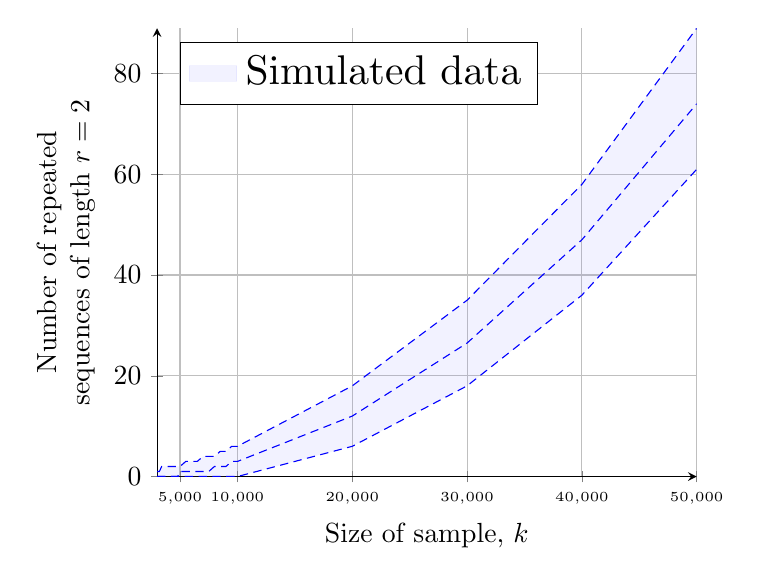
\begin{tikzpicture}
\begin{axis}[
    axis lines=left, %xtick=\empty, ytick=\empty.
    grid=both,
    scaled x ticks = false,
    xticklabel style = {font=\tiny},
    xtick = {2000,5000,10000,20000,30000,40000,50000},
    %xticklabels = {$2000$,$5000$,$10,000$,$20,000$,$30,000$,$40,000$},
    ylabel style = {align=center},
	xlabel = {Size of sample, $k$},
        ylabel = {Number of repeated\\ sequences of length $r=2$},
    legend style={at={(axis cs:5000,80)},anchor=west,cells={align=center},nodes={scale=1.5}},
]
% Include the simulated data
\addplot[forget plot,densely dashed,color=blue,name path=down]coordinates {
	(3000.0000	,	0.0000)
	(3200.0000	,	0.0000)
	(3400.0000	,	0.0000)
	(3600.0000	,	0.0000)
	(3800.0000	,	0.0000)
	(4000.0000	,	0.0000)
	(4200.0000	,	0.0000)
	(4400.0000	,	0.0000)
	(4600.0000	,	0.0000)
	(4800.0000	,	0.0000)
	(5000.0000	,	0.0000)
	(5500.0000	,	0.0000)
	(6000.0000	,	0.0000)
	(6500.0000	,	0.0000)
	(7000.0000	,	0.0000)
	(7500.0000	,	0.0000)
	(8000.0000	,	0.0000)
	(8500.0000	,	0.0000)
	(9000.0000	,	0.0000)
	(9500.0000	,	0.0000)
	(10000.0000	,	0.0000)
	(20000.0000	,	6.0000)
	(30000.0000	,	18.0000)
	(40000.0000	,	36.0000)
	(50000.0000	,	61.0000)
};
\addplot[forget plot,densely dashed,color=blue]coordinates {
	(3000.0000	,	0.0000)
	(3200.0000	,	0.0000)
	(3400.0000	,	0.0000)
	(3600.0000	,	0.0000)
	(3800.0000	,	0.0000)
	(4000.0000	,	0.0000)
	(4200.0000	,	0.0000)
	(4400.0000	,	0.0000)
	(4600.0000	,	0.0000)
	(4800.0000	,	0.0000)
	(5000.0000	,	1.0000)
	(5500.0000	,	1.0000)
	(6000.0000	,	1.0000)
	(6500.0000	,	1.0000)
	(7000.0000	,	1.0000)
	(7500.0000	,	1.0000)
	(8000.0000	,	2.0000)
	(8500.0000	,	2.0000)
	(9000.0000	,	2.0000)
	(9500.0000	,	3.0000)
	(10000.0000	,	3.0000)
	(20000.0000	,	12.0000)
	(30000.0000	,	26.5000)
	(40000.0000	,	47.0000)
	(50000.0000	,	74.0000)
};
\addplot[forget plot,densely dashed,color=blue,name path=up]coordinates {
	(3000.0000	,	1.0000)
	(3200.0000	,	1.0000)
	(3400.0000	,	2.0000)
	(3600.0000	,	2.0000)
	(3800.0000	,	2.0000)
	(4000.0000	,	2.0000)
	(4200.0000	,	2.0000)
	(4400.0000	,	2.0000)
	(4600.0000	,	2.0000)
	(4800.0000	,	2.0000)
	(5000.0000	,	2.0000)
	(5500.0000	,	3.0000)
	(6000.0000	,	3.0000)
	(6500.0000	,	3.0000)
	(7000.0000	,	4.0000)
	(7500.0000	,	4.0000)
	(8000.0000	,	4.0000)
	(8500.0000	,	5.0000)
	(9000.0000	,	5.0000)
	(9500.0000	,	6.0000)
	(10000.0000	,	6.0000)
	(20000.0000	,	18.0000)
	(30000.0000	,	35.0000)
	(40000.0000	,	58.0000)
	(50000.0000	,	89.0000)
};
\addplot[blue!50,opacity=0.1] fill between[of=up and down];
\addlegendentry{Simulated data}
\end{axis}
\end{tikzpicture}
% E_U
\begin{tikzpicture}
\begin{axis}[
    axis lines=left, %xtick=\empty, ytick=\empty.
    grid=both,
    scaled x ticks = false,
    xticklabel style = {font=\tiny},
    scaled y ticks = false,
    %yticklabel style = {font=\tiny},
    ymax = 220,
    ymin =0,
    xmin = 3000,
    xmax = 15000,
    ytick = {10,20,30,40,50,75,100,125,150,175,200},
    ylabel style = {align=center},
	xlabel = {Size of sample, $k$},
        ylabel = {Number of repeated\\ sequences of length $r=2$},
    legend style={anchor=west,at={(axis cs:3500,180)},cells={align=center},nodes={scale=1.5}},
]
% Include the theoretical values
%\addplot[color=magenta!50]coordinates {
	(3000.0000	,	0.4818)
	(3200.0000	,	0.5336)
	(3400.0000	,	0.5841)
	(3600.0000	,	0.6322)
	(3800.0000	,	0.6770)
	(4000.0000	,	0.7177)
	(4200.0000	,	0.7535)
	(4400.0000	,	0.7838)
	(4600.0000	,	0.8079)
	(4800.0000	,	0.8254)
	(5000.0000	,	0.8361)
	(5500.0000	,	0.8330)
	(6000.0000	,	0.7898)
	(6500.0000	,	0.7143)
	(7000.0000	,	0.6175)
	(7500.0000	,	0.5109)
	(8000.0000	,	0.4052)
	(8500.0000	,	0.3083)
	(9000.0000	,	0.2254)
	(9500.0000	,	0.1584)
	(10000.0000	,	0.1071)
	(20000.0000	,	0.0000)
	(30000.0000	,	0.0000)
	(40000.0000	,	0.0000)
	(50000.0000	,	0.0000)
};
\addlegendentry{$E_L$} % Lower
\addplot[color=magenta]coordinates {
	(3000.0000	,	0.8229)
	(3200.0000	,	0.9812)
	(3400.0000	,	1.1618)
	(3600.0000	,	1.3667)
	(3800.0000	,	1.5985)
	(4000.0000	,	1.8596)
	(4200.0000	,	2.1526)
	(4400.0000	,	2.4805)
	(4600.0000	,	2.8460)
	(4800.0000	,	3.2522)
	(5000.0000	,	3.7023)
	(5500.0000	,	5.0420)
	(6000.0000	,	6.7330)
	(6500.0000	,	8.8362)
	(7000.0000	,	11.4180)
	(7500.0000	,	14.5498)
	(8000.0000	,	18.3083)
	(8500.0000	,	22.7755)
	(9000.0000	,	28.0387)
	(9500.0000	,	34.1904)
	(10000.0000	,	41.3284)
	(20000.0000	,	587.9817)
	(30000.0000	,	2900.0470)
	(40000.0000	,	9061.6718)
	(50000.0000	,	21970.8243)
};
\addlegendentry{$E_U$} % Upper
\end{axis}
  \end{tikzpicture}
% E_L
\begin{tikzpicture}
\begin{axis}[
    axis lines=left, %xtick=\empty, ytick=\empty.
    grid=both,
    xmin = 3000,
    xmax = 11000,
    scaled x ticks = false,
    xticklabel style = {font=\tiny},
    xtick = {2000,4000,6000,8000,10000},
    ylabel style = {align=center},
	xlabel = {Size of sample, $k$},
        ylabel = {Number of repeated\\ sequences of length $r=2$},
    legend style={anchor=west,at={(axis cs:9000,0.7)},cells={align=center},nodes={scale=1.5}},
]
% Include the theoretical values
\addplot[color=magenta!50]coordinates {
	(3000.0000	,	0.4818)
	(3200.0000	,	0.5336)
	(3400.0000	,	0.5841)
	(3600.0000	,	0.6322)
	(3800.0000	,	0.6770)
	(4000.0000	,	0.7177)
	(4200.0000	,	0.7535)
	(4400.0000	,	0.7838)
	(4600.0000	,	0.8079)
	(4800.0000	,	0.8254)
	(5000.0000	,	0.8361)
	(5500.0000	,	0.8330)
	(6000.0000	,	0.7898)
	(6500.0000	,	0.7143)
	(7000.0000	,	0.6175)
	(7500.0000	,	0.5109)
	(8000.0000	,	0.4052)
	(8500.0000	,	0.3083)
	(9000.0000	,	0.2254)
	(9500.0000	,	0.1584)
	(10000.0000	,	0.1071)
	(20000.0000	,	0.0000)
	(30000.0000	,	0.0000)
	(40000.0000	,	0.0000)
	(50000.0000	,	0.0000)
};
\addlegendentry{$E_L$} % Lower
%\addplot[color=magenta]coordinates {
	(3000.0000	,	0.8229)
	(3200.0000	,	0.9812)
	(3400.0000	,	1.1618)
	(3600.0000	,	1.3667)
	(3800.0000	,	1.5985)
	(4000.0000	,	1.8596)
	(4200.0000	,	2.1526)
	(4400.0000	,	2.4805)
	(4600.0000	,	2.8460)
	(4800.0000	,	3.2522)
	(5000.0000	,	3.7023)
	(5500.0000	,	5.0420)
	(6000.0000	,	6.7330)
	(6500.0000	,	8.8362)
	(7000.0000	,	11.4180)
	(7500.0000	,	14.5498)
	(8000.0000	,	18.3083)
	(8500.0000	,	22.7755)
	(9000.0000	,	28.0387)
	(9500.0000	,	34.1904)
	(10000.0000	,	41.3284)
	(20000.0000	,	587.9817)
	(30000.0000	,	2900.0470)
	(40000.0000	,	9061.6718)
	(50000.0000	,	21970.8243)
};
\addlegendentry{$E_U$} % Upper
\end{axis}
\end{tikzpicture}


\end{document}
